\chapter{Sobre la complejidad de H y el ruido}

En este capítulo, trataremos la dificultad que introduce la aparición de
ruido en las etiquetas a la hora de elegir la clase de funciones más adecuadas.

\section{Dibujar gráficas de nubes de puntos simuladas}

\subsection{Uniformemente distribuidos}

\textbf{Considere $N = 50$, $\dim = 2$, $rango = [-50, 50]$ con
\mintinline{python}{simula_unif(N, dim, rango)}}

\begin{figure}[H]
\centering
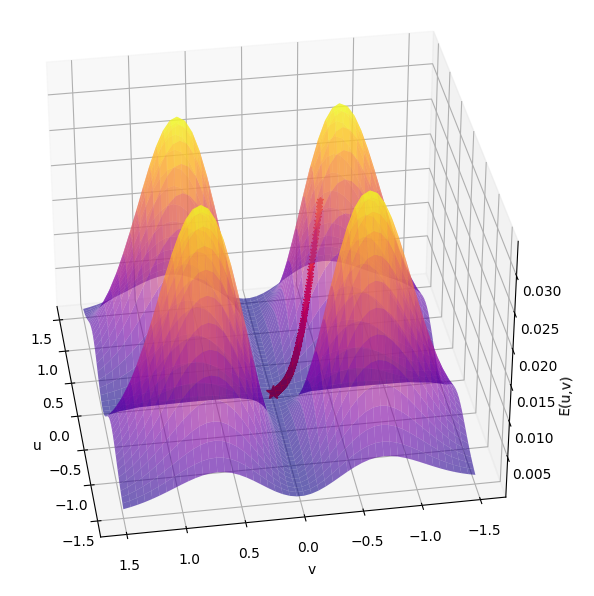
\includegraphics[width=0.5\textwidth]{Figure_1.png}
\caption{Gráfica de nube de puntos uniformemente distribuidos}
\end{figure}

\hfill \break

\subsection{Siguiendo distribución gaussiana de media \texorpdfstring{$0$} y varianza dada}

\textbf{Considere $N = 50$, $dim = 2$ y $sigma = [5, 7]$ con 
\mintinline{python}{simula_gauss(N, dim, sigma)}}

\begin{figure}[H]
\centering
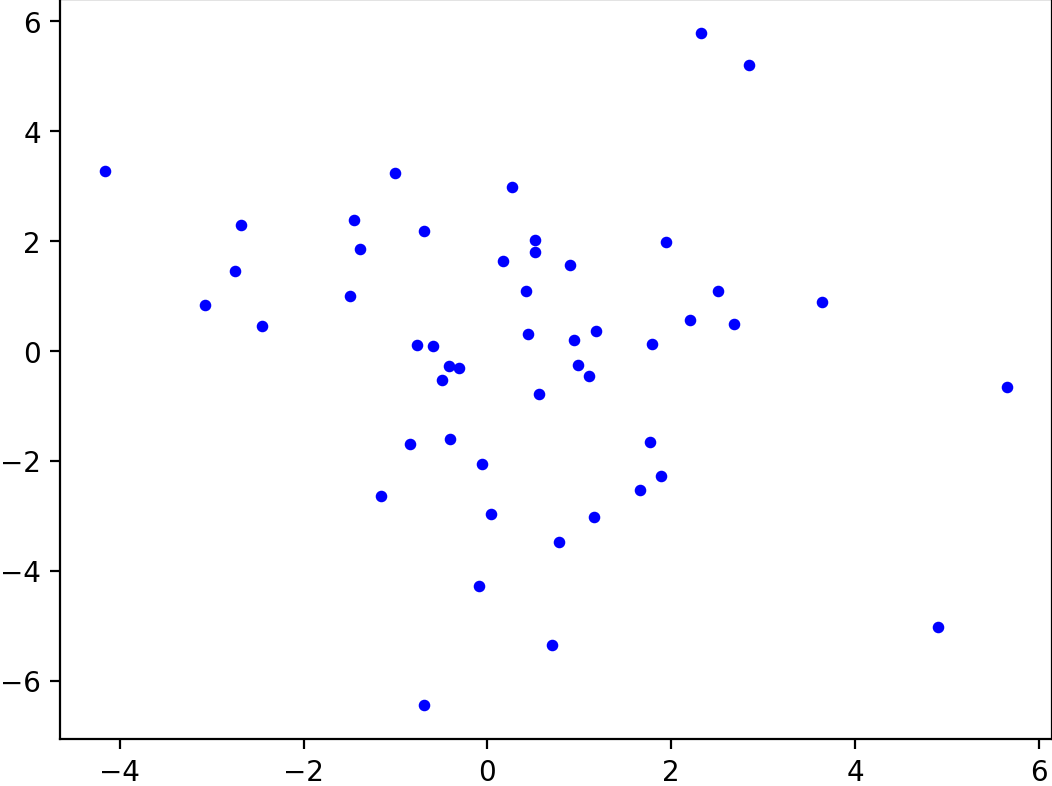
\includegraphics[width=0.5\textwidth]{Figure_2.png}
\caption{Gráfica de nube de puntos en distribución gaussiana.}
\end{figure}

Al seguir una distribución normal de media cero y varianza sigma, los puntos se
acumulan en $\left[ -\sqrt{5}, \sqrt{5} \right] \times \left[-\sqrt{7}, \sqrt{7}\right]  \approx [-2.2, 2.2] \times [-2.6, 2.6]$

\section{Ejercicio 2}

Vamos a valorar la influencia del ruido en la selección de la complejidad de la
clase de funciones.  Con ayuda de la función
\mintinline{python}{simula_unif(100, 2, [-50, 50])} generamos una muestra de
puntos 2D a los que vamos añadir una etiqueta usando el signo de la función 
$f(x, y) = y - ax - b$, es decir el signo de cada punto con respecto a la
recta simulada con \mintinline{python}{simula_recta()}.  

\subsection{Dibujo de puntos con etiqueta y recta usada}

Dibujamos un gráfico 2D con los puntos clasificados por etiquetas junto
con la recta usada para etiquetar. 

\begin{figure}[H]
\centering
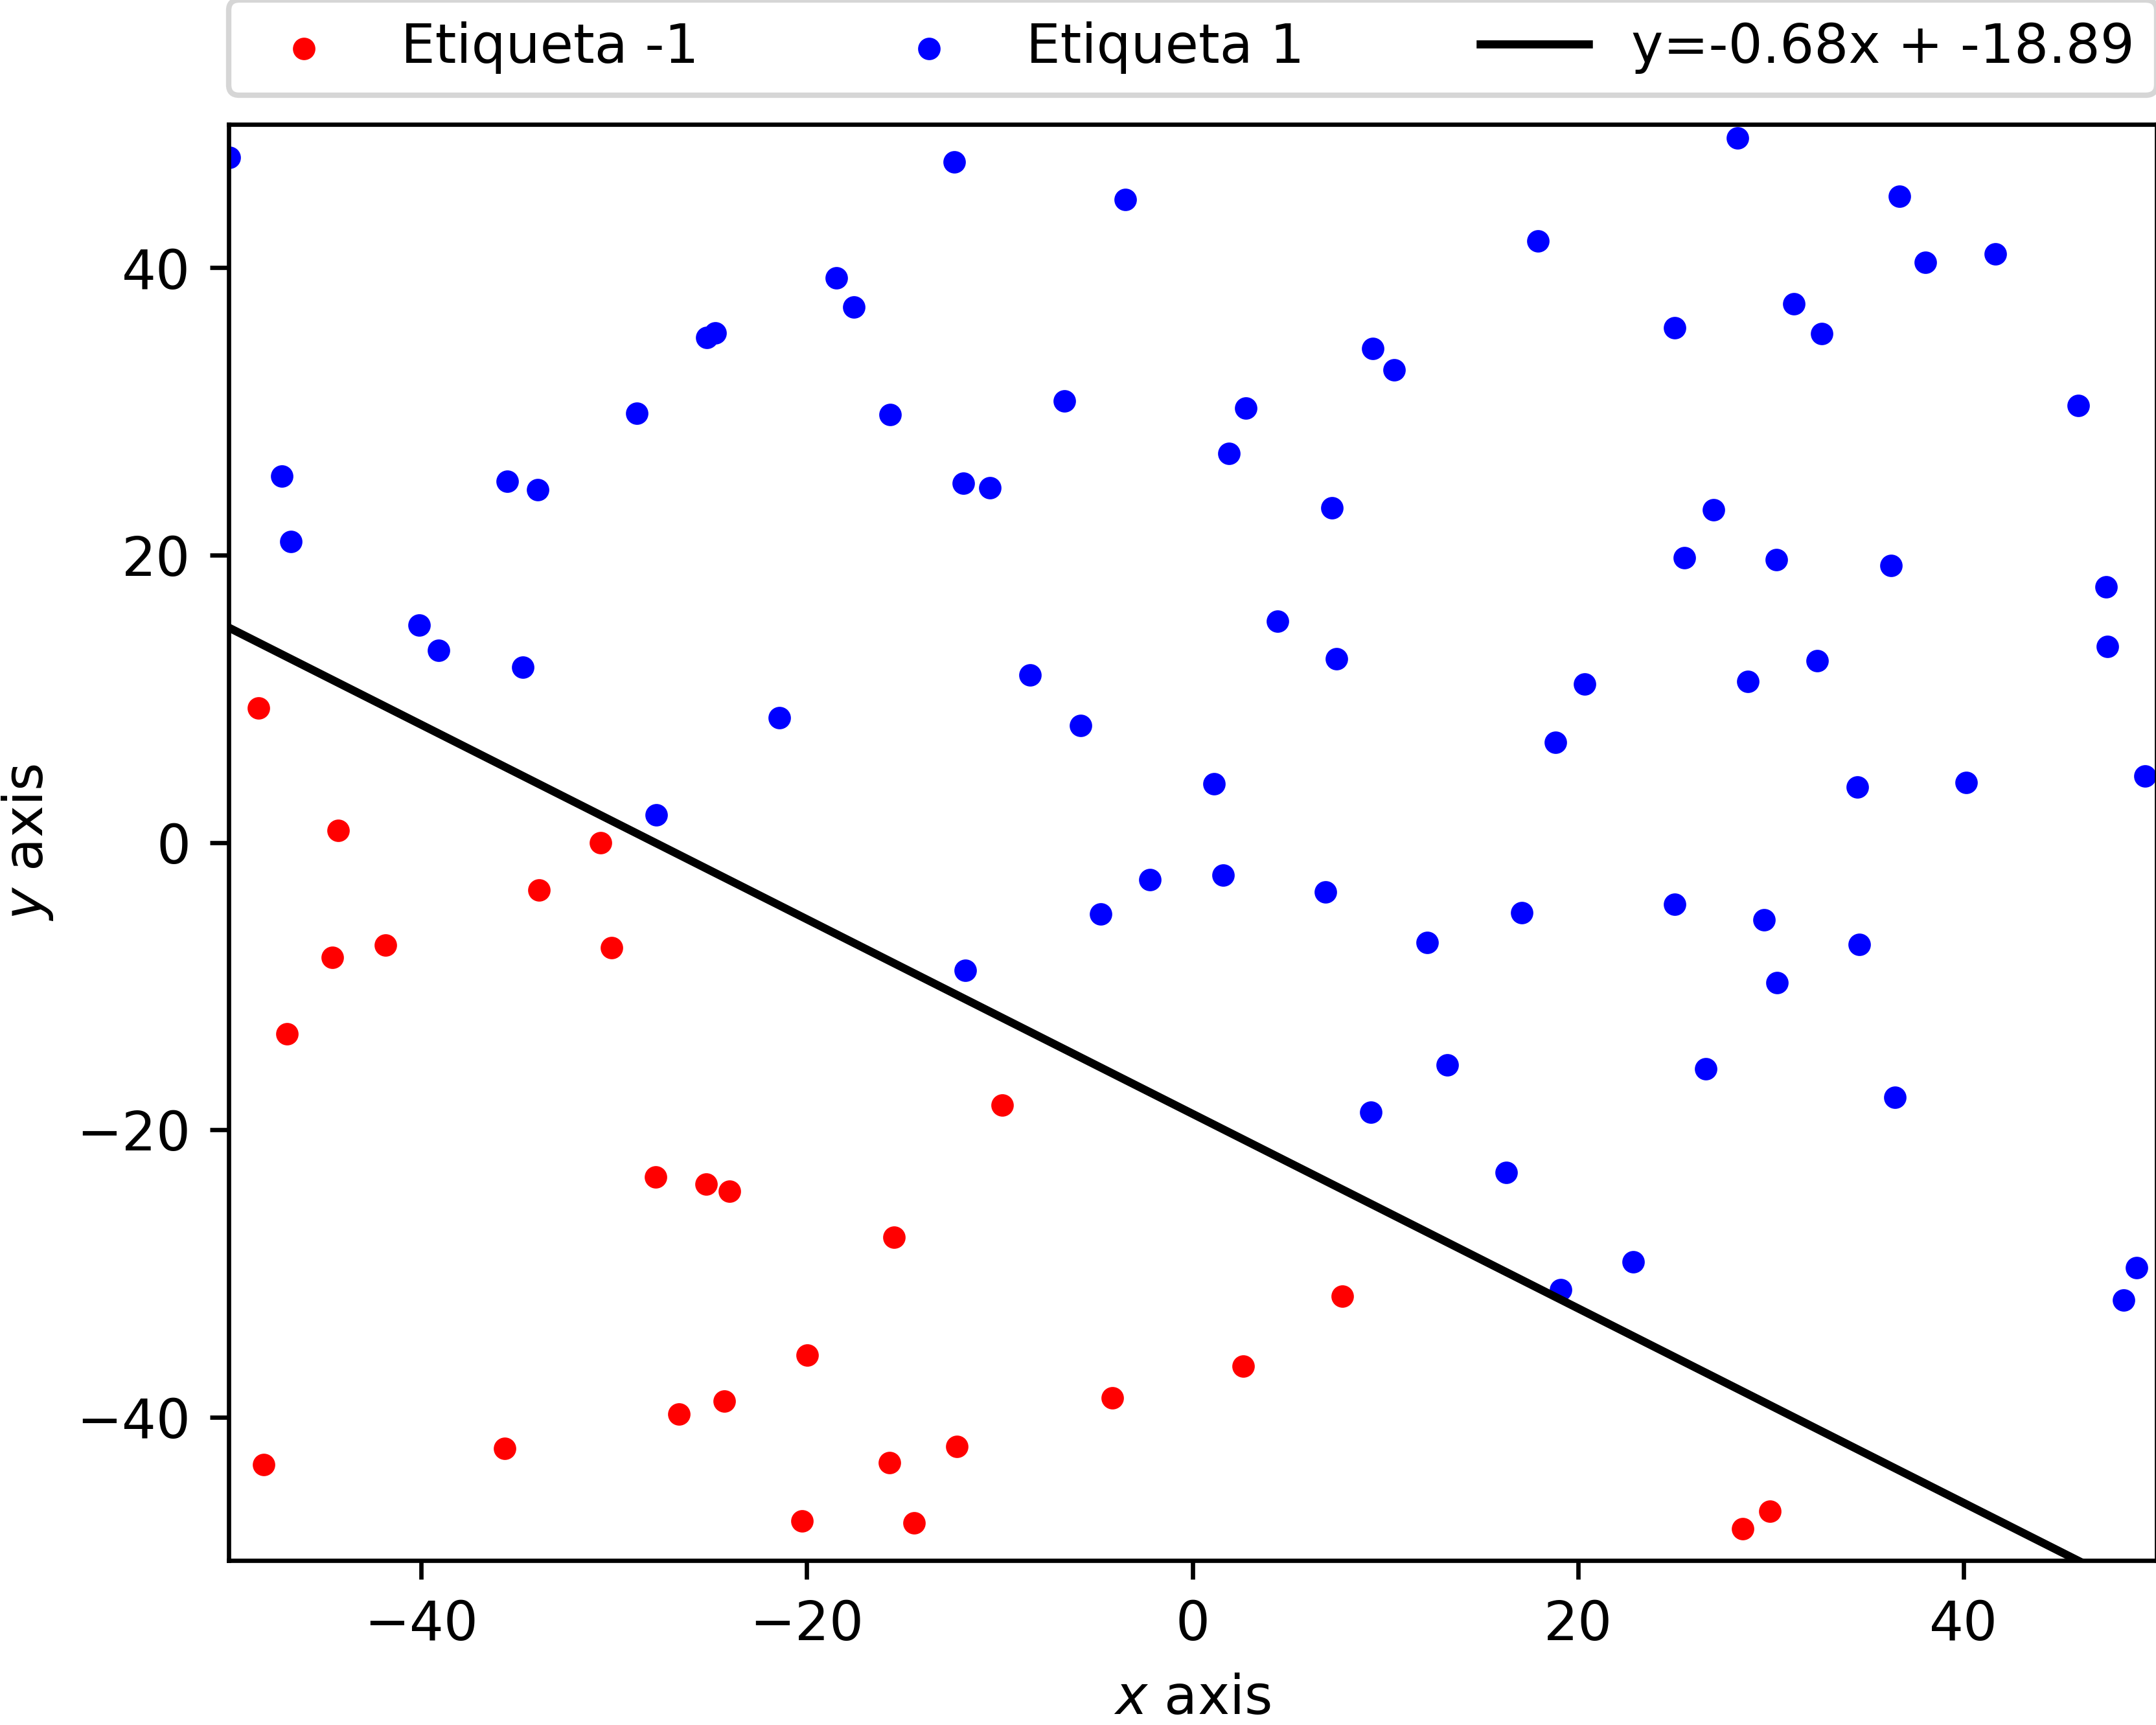
\includegraphics[width=0.5\textwidth]{Figure_3.png}
\caption{Etiquetado de puntos uniformemente distribuidos según recta.}
\end{figure}

Es claro que si usamos una recta para etiquetar los puntos en dos clases,
estos datos está bien clasificados por esta recta.

\subsection{Añadir ruido aleatorio}

Modifique de forma aleatoria un $10\%$ de las etiquetas positivas y otro $10\%$
de las negativas y guarde los puntos con sus nuevas etiquetas. Dibuje de nuevo
la gráfica anterior. Ahora habrá puntos mal clasificados respecto de la recta.  

\begin{figure}[H]
\centering
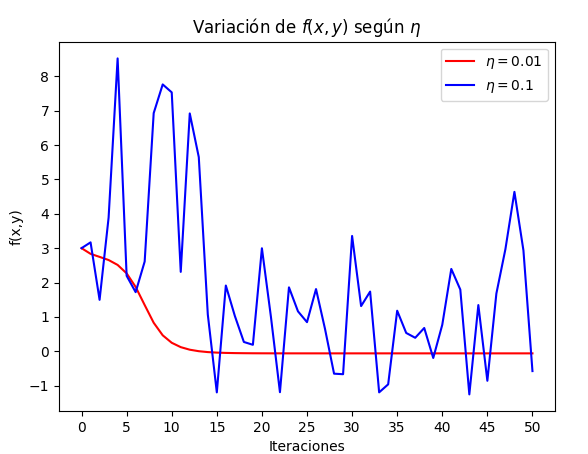
\includegraphics[width=0.5\textwidth]{Figure_4.png}
\caption{Nube de puntos anterior con 10\% de ruido en cada etiqueta.}
\end{figure}

En efecto, $3$ puntos con etiqueta $-1$ (rojos) ahora tienen etiqueta $1$
(son azules). Esto es el $10\%$ del total ($27$) redondeado.

\subsection{Otras fronteras de clasificación}

Supongamos ahora que las siguientes funciones ($f_1, f_2, f_3, f_4$)
definen la frontera de clasificación de los puntos de la muestra en 
lugar de una recta.

\textbf{Visualizar el etiquetado generado en el apartado 2b junto con la gráfica de cada
una de las funciones.  Comparar las regiones positivas y negativas de estas
nuevas funciones con las obtenidas en el caso de la recta.  Argumente si estas
funciones más complejas son mejores clasificadores que la función lineal.
Observe las gráficas y diga qué consecuencias extrae sobre la influencia de la
modificación de etiquetas en el proceso de aprendizaje. Explique el
razonamiento.}

\hfill \break

Usando la función \mintinline{python}{plot_datos_cuad} proporcionada en
la plantilla de código, podemos visualizar y comparar las regiones positivas
y negativas (azul y rojo respectivamente) que define la frontera dada por
$f_i(x,y) = 0$ con $i=1,2,3,4$.

\subsubsection{Circunferencia y Elipse}

\begin{multicols}{2}
\begin{itemize}
\item $f_1(x,y) = (x - 10)^2 + (y - 20)^2 - 400$
\item $f_2(x,y) = \frac{(x + 10)^2}{2} + (y - 20)^2 - 400$
\end{itemize}
\end{multicols}

\begin{figure}[H]
  \begin{minipage}[b]{.5\linewidth}
    \centering
    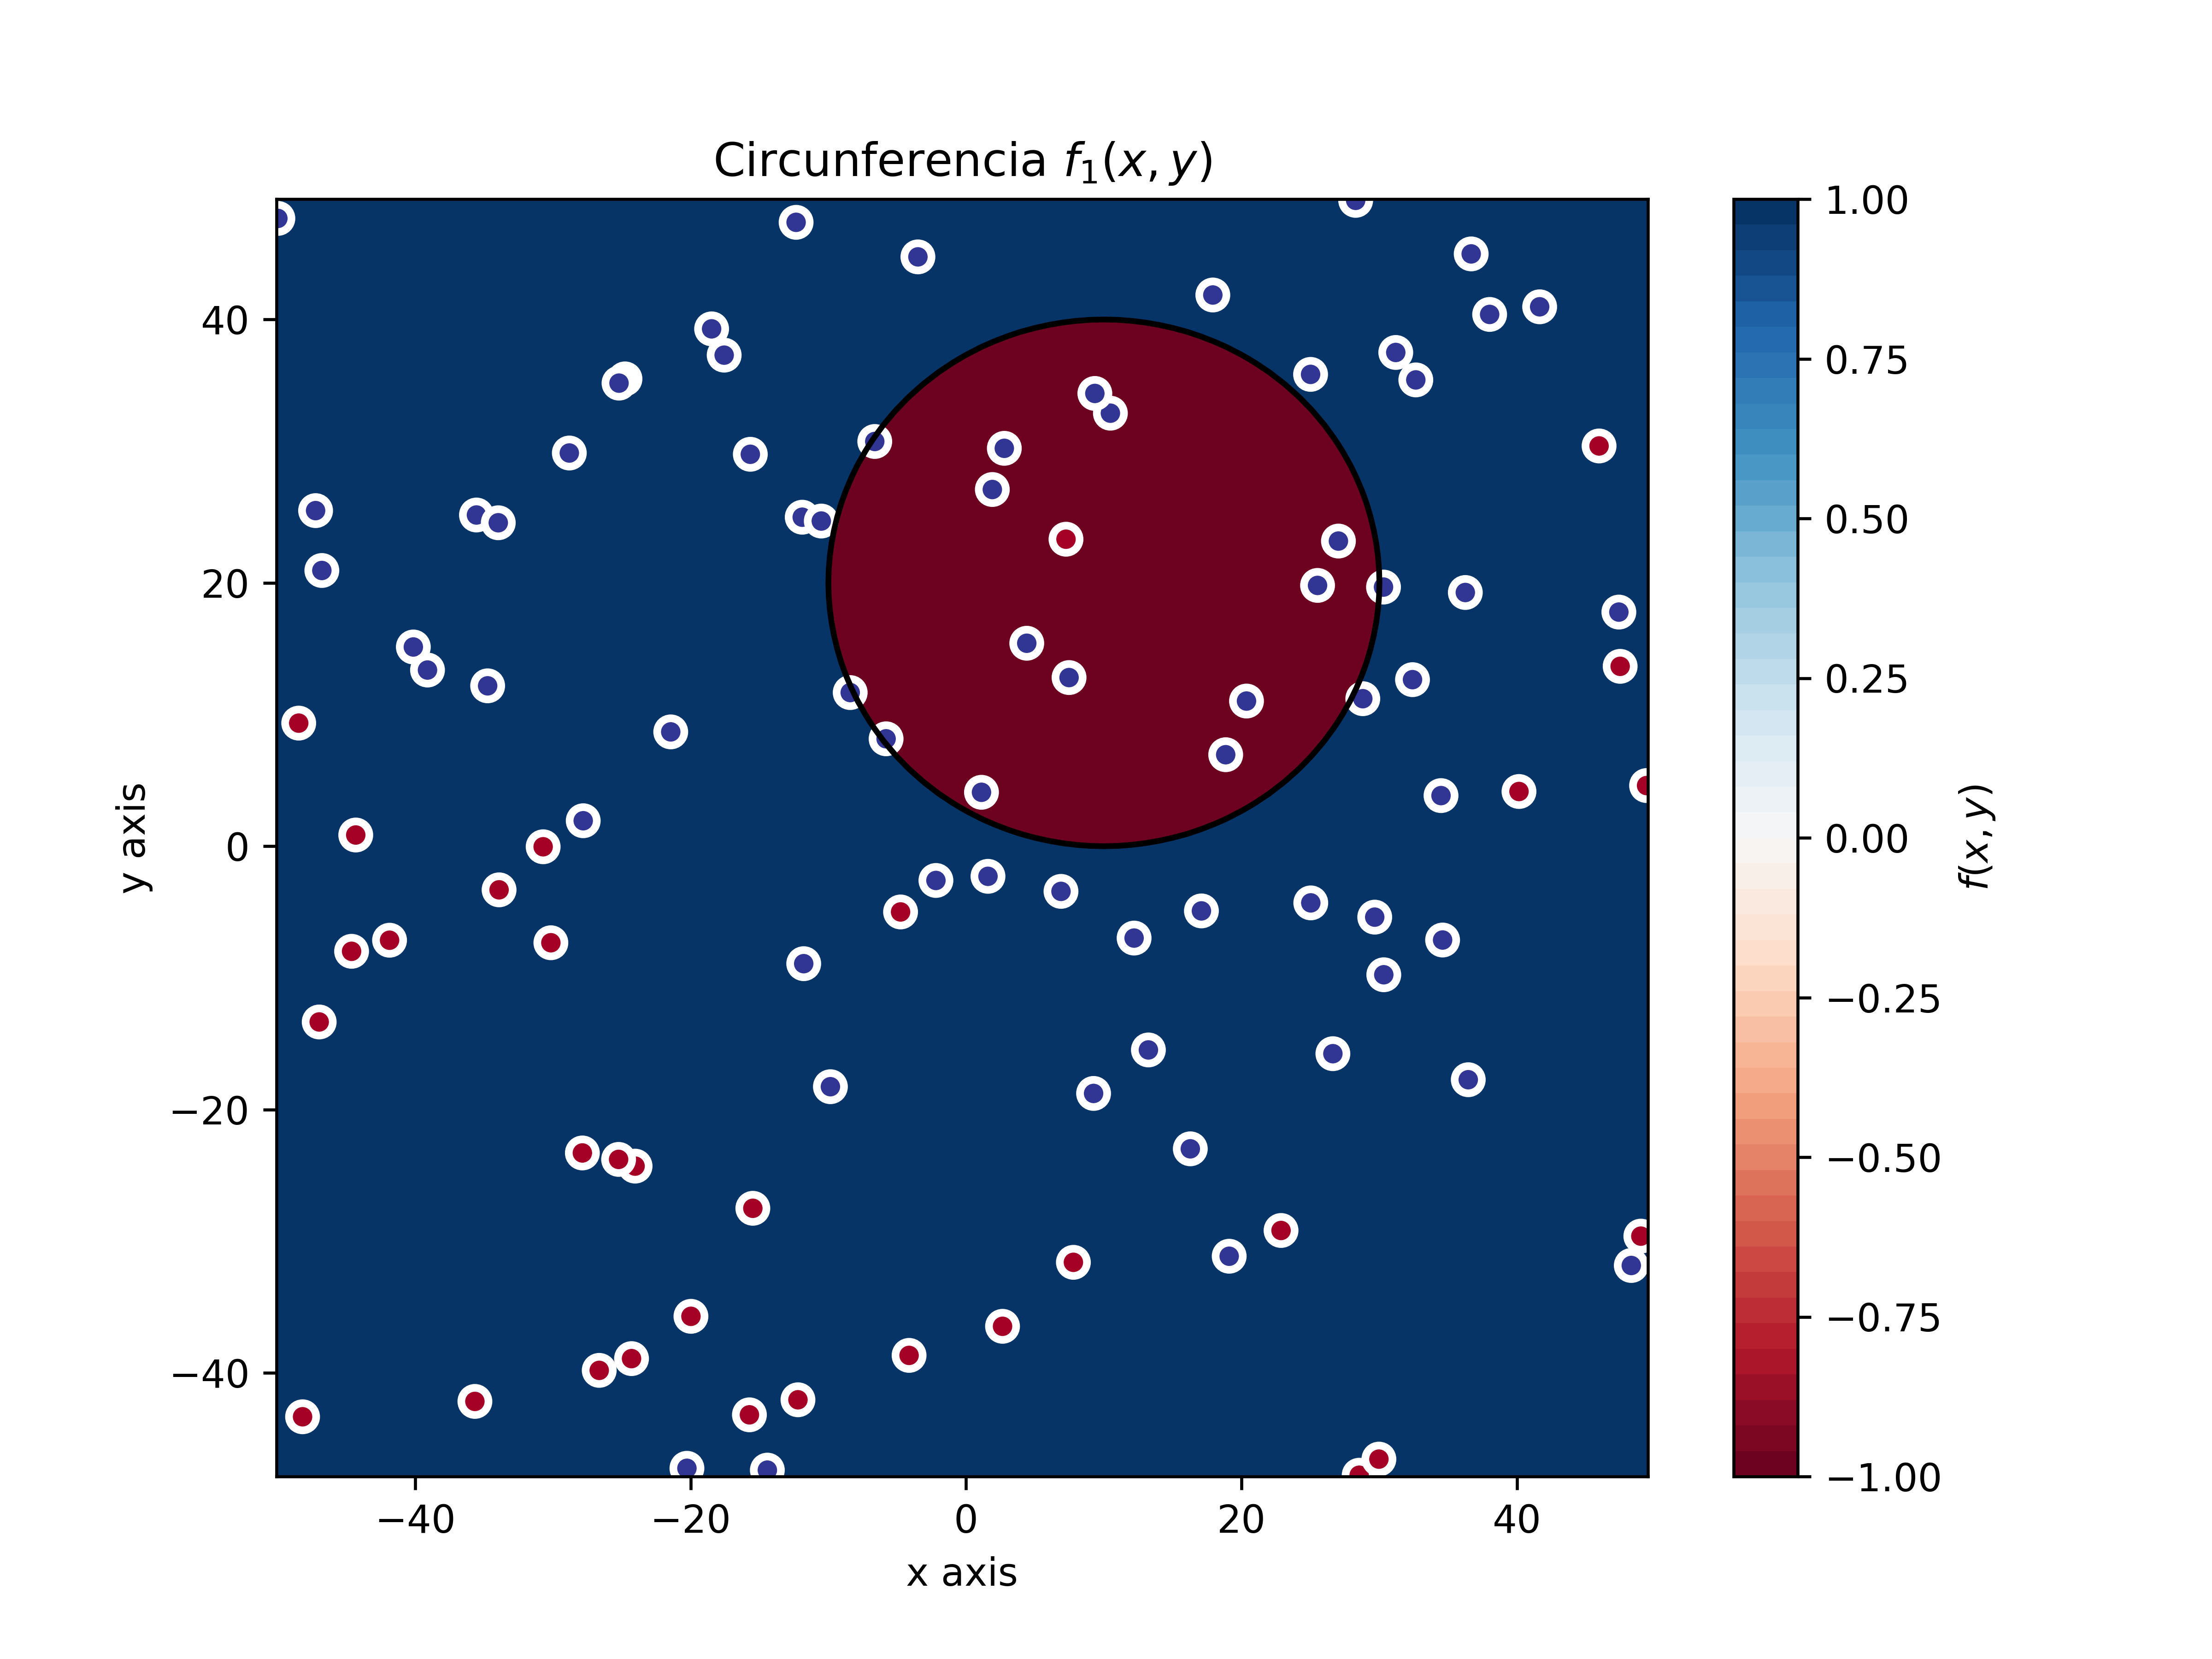
\includegraphics[width=0.9\textwidth]{Figure_5}
    \subcaption{Muestra clasificada por circunferencia $f_1$}\label{subfig-1:dummy}
  \end{minipage}
  \hfill \hfill
  \begin{minipage}[b]{.5\linewidth}
    \centering
    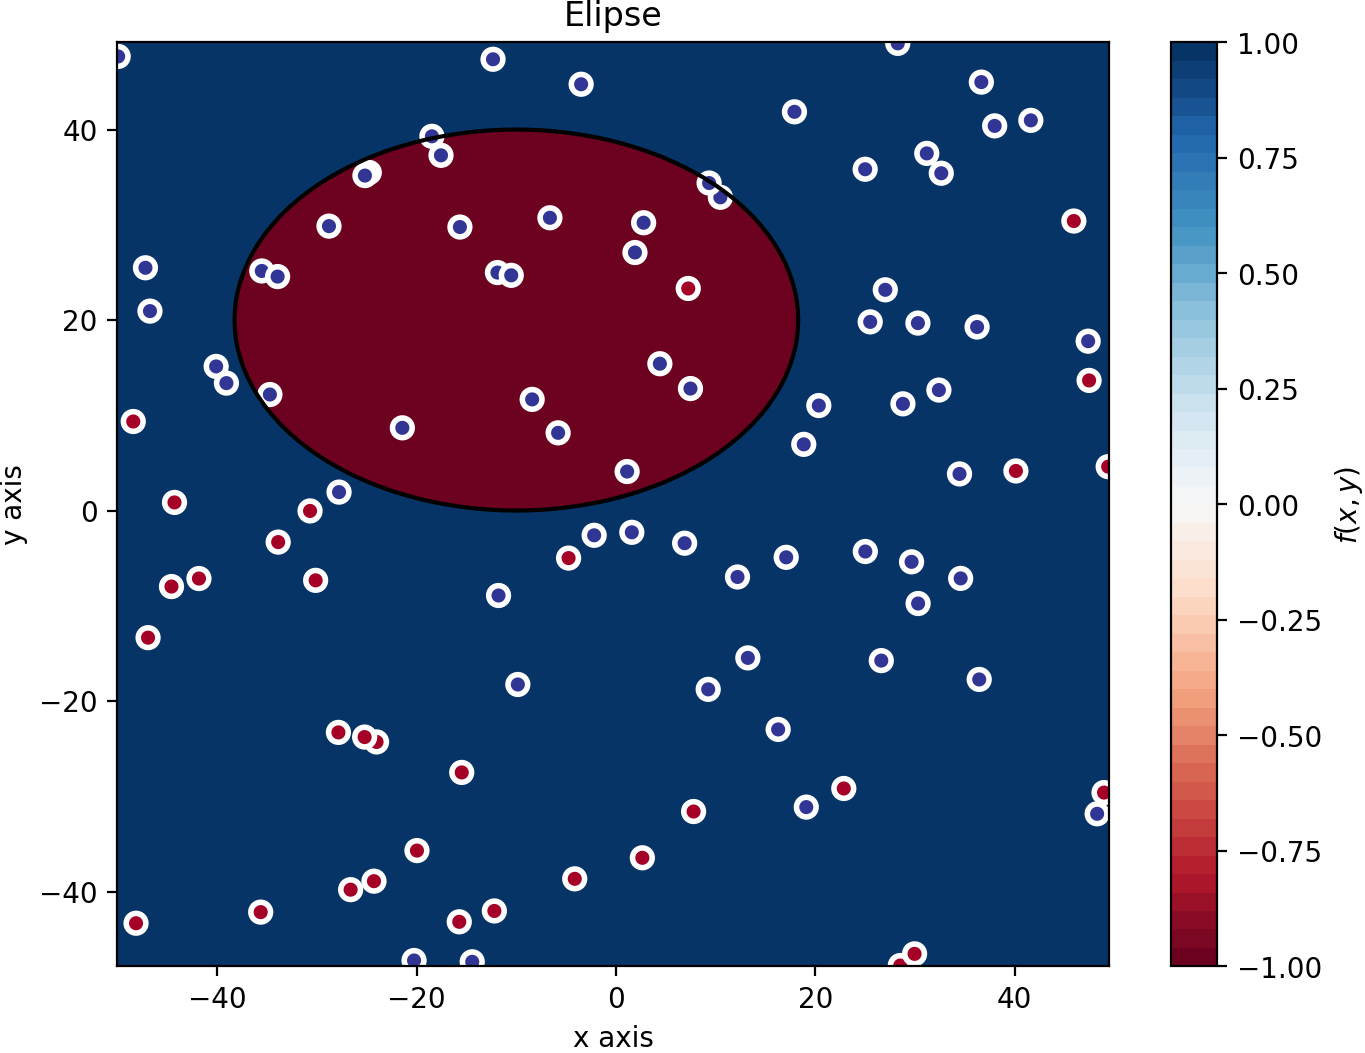
\includegraphics[width=0.9\textwidth]{Figure_6}
    \subcaption{Muestra clasificada por elipse $f_2$}\label{subfig-2:dummy}
  \end{minipage}
%  \caption{Dummy figure}
  \label{fig:dummy}
\end{figure}

\hfill \break

\subsubsection{Hipérbola y Parábola}

\begin{multicols}{2}
\begin{itemize}
\item $f_3(x,y) = \frac{(x - 10)^2}{2} - (y + 20)^2 - 400$
\item $f_4(x,y) = y - 20x^2 - 5x + 3$
\end{itemize}
\end{multicols}

\begin{figure}[H]
  \begin{minipage}[b]{.5\linewidth}
    \centering
    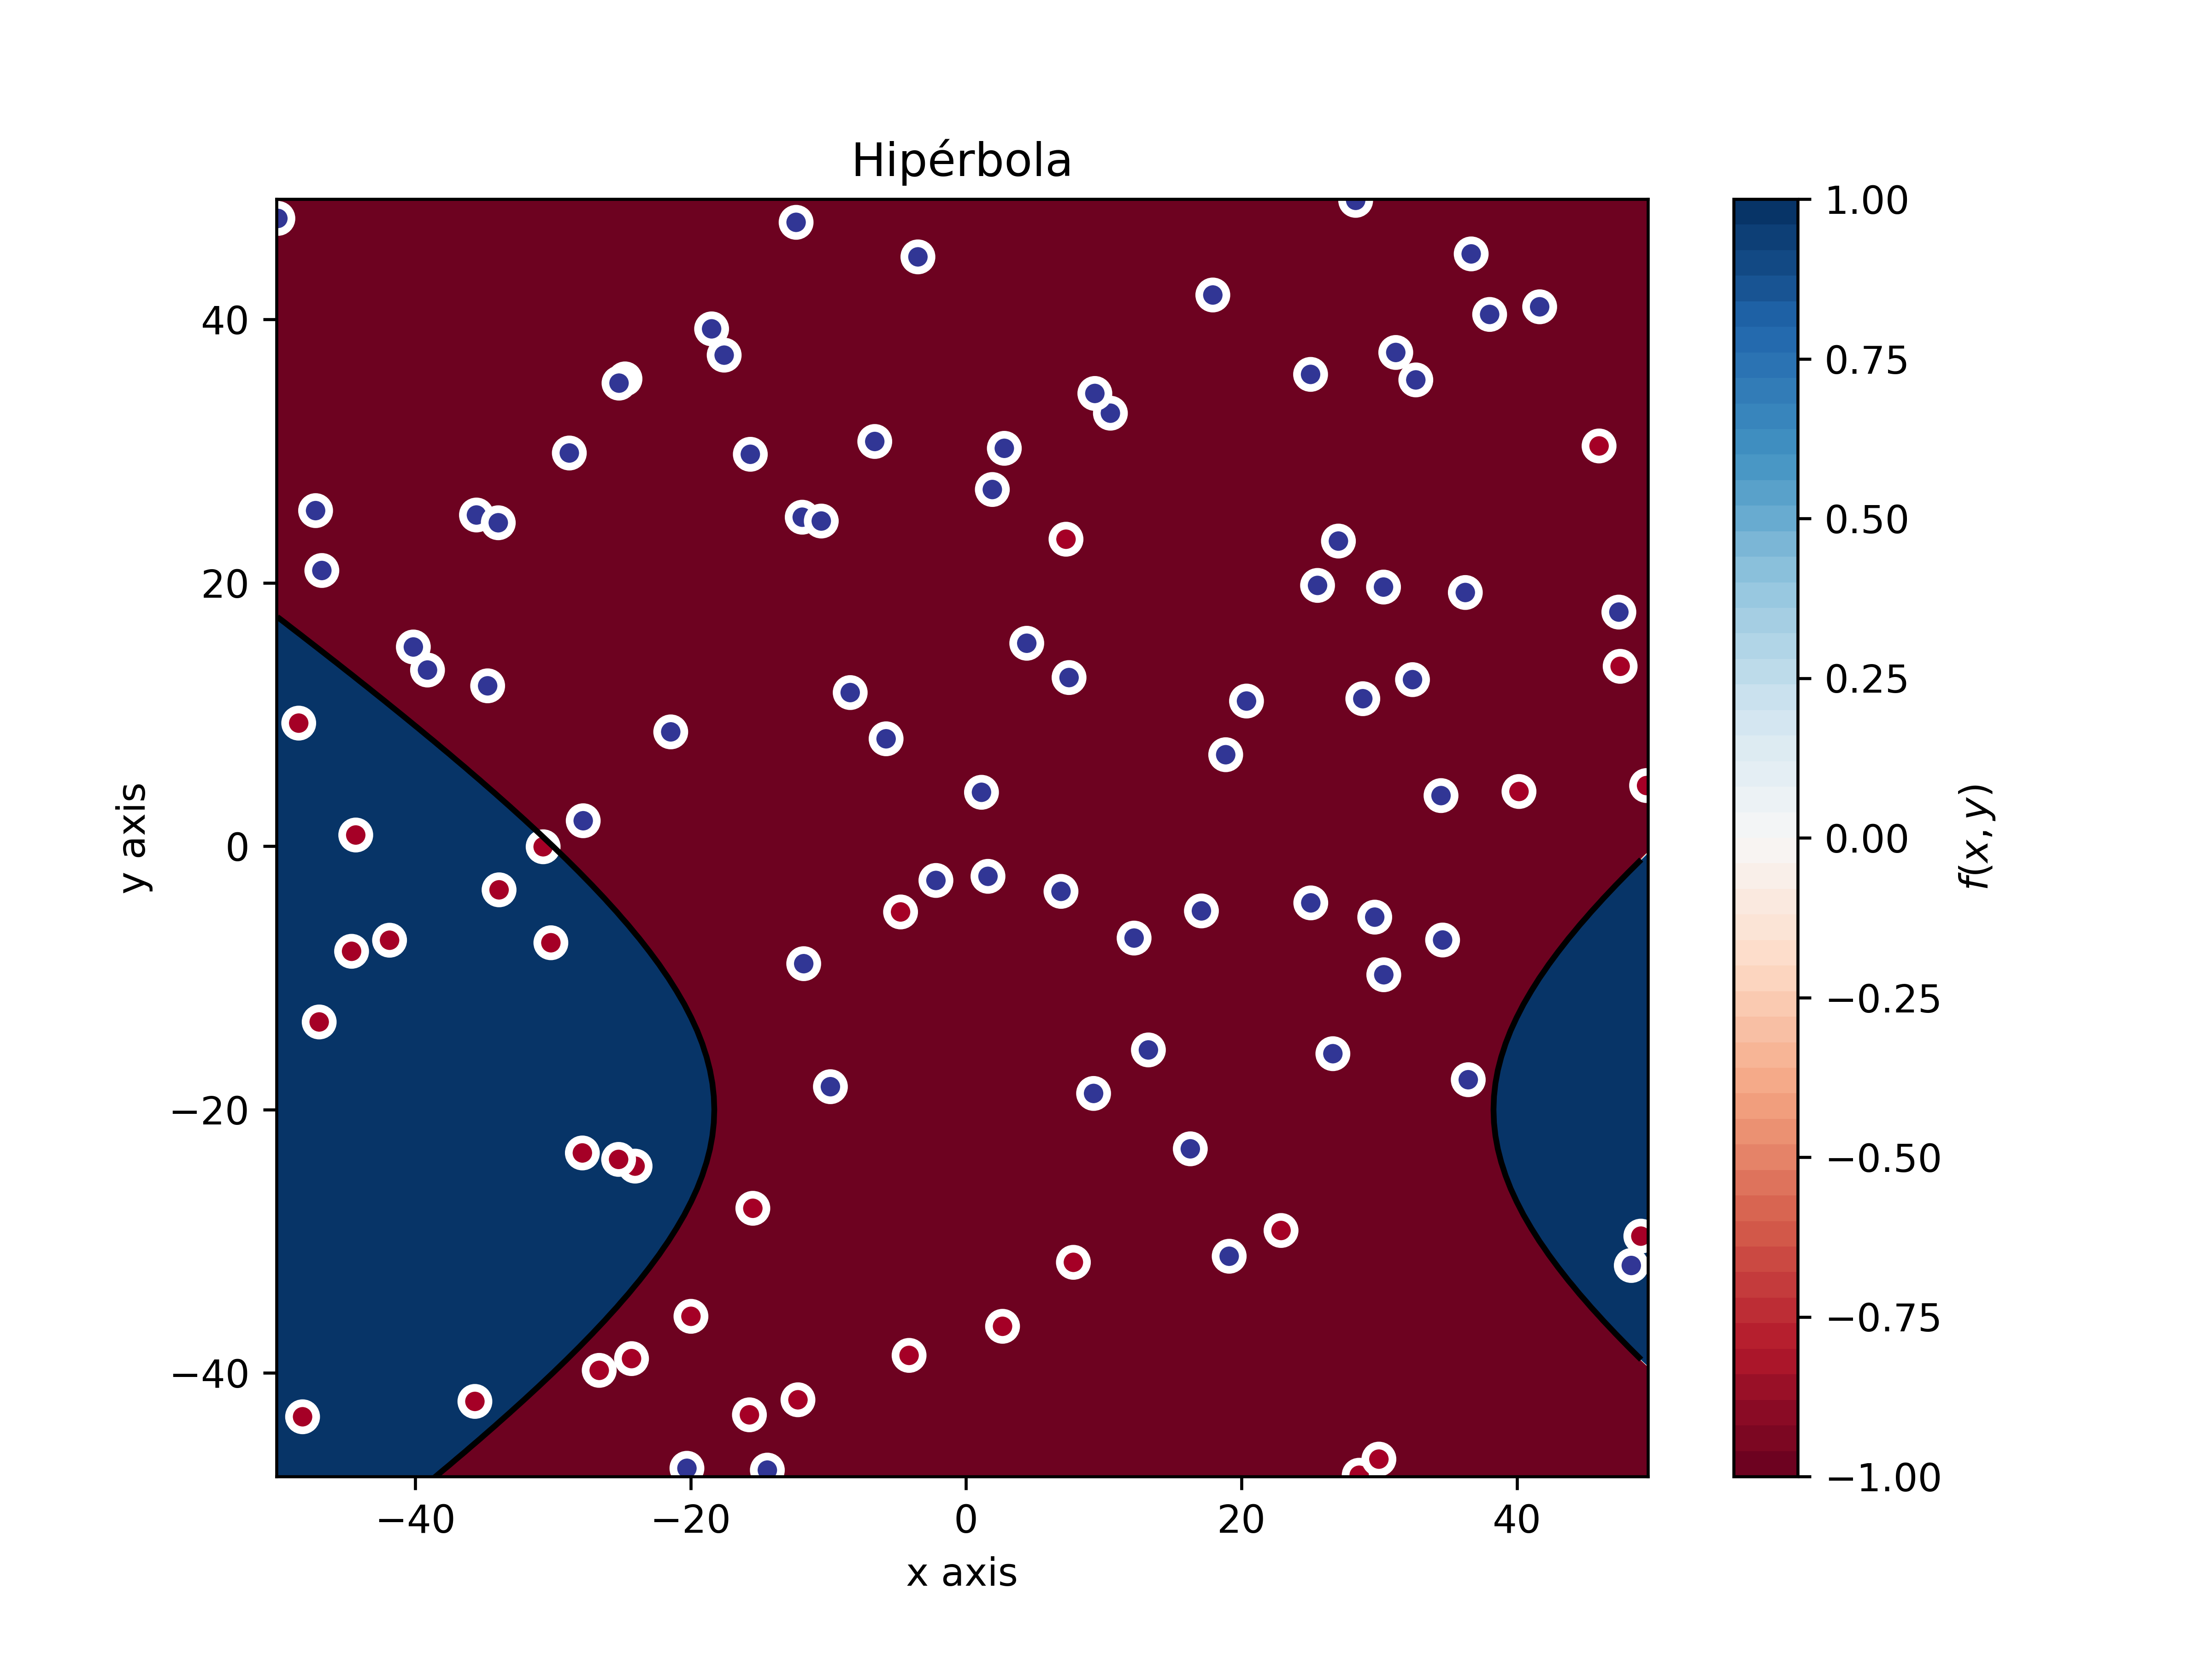
\includegraphics[width=0.9\textwidth]{Figure_7}
    \subcaption{Muestra clasificada por hipérbola $f_3$}\label{subfig-3:dummy}
  \end{minipage}
  \hfill \hfill
  \begin{minipage}[b]{.5\linewidth}
    \centering
    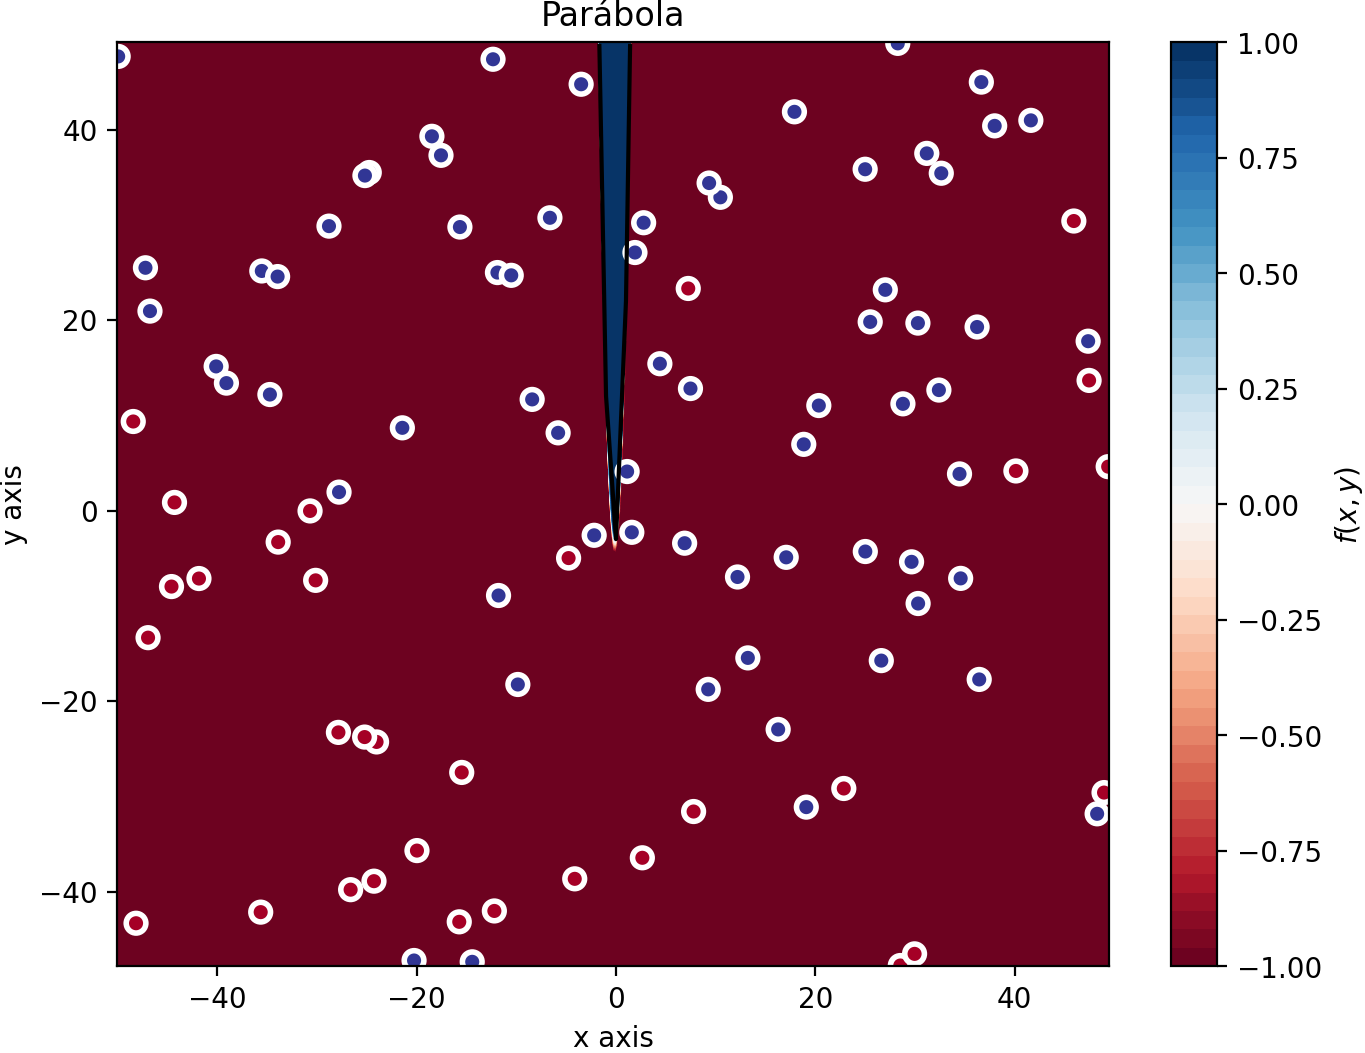
\includegraphics[width=0.9\textwidth]{Figure_8}
    \subcaption{Muestra clasificada por parábola $f_4$}\label{subfig-4:dummy}
  \end{minipage}
%  \caption{Dummy figure}
  \label{fig:dummy2}
\end{figure}

Si calculamos el error de clasificación en cada uno de los casos obtenemos:

\begin{table}[!ht]
%    \caption {Valor mínimo para $\eta = 0.1$} \label{tab:title} 
    \centering
    \begin{tabular}{cc}
    \toprule
        $f_i$ & Error de clasificación (\%) \\ \midrule
        Recta $f$            & $10\%$ \\
        Circunferencia $f_1$ & $44\%$  \\ 
        Elipse $f_2$         & $52\%$  \\
        Hipérbola $f_3$      & $81\%$  \\
        Parábola $f_4$       & $68\%$ \\ \bottomrule
    \end{tabular}
\end{table}

Podemos confirmar lo que se podía intuir por las grafícas obtenidas.
A pesar de ser funciones más complejas que la lineal, no son mejores
clasificadores. 

En cuanto a la influencia del ruido, no es posible obtener un mejor
clasificador que la recta $f$. Esto se debe a que el ruido ha sido generado
aleatoriamente y que es la propia recta $f$ la que se ha usado para
etiquetar. Así, el $10\%$ es cota inferior del de error de clasificación para
distinto $\mathcal{H}$.

De hecho, para funciones demasiado complejas es probable que tengamos
un problema de \textbf{sobreajuste} (overfitting) impidiendo una buena
generalización (alto valor de $E_{out}$).